\chapter{Blockchain Scalability}

\section{Bottlenecks in Scalability}
A blockchain's ability to scale is often measured by the amount of transactions it can verify per second. A block gets appended to the Ethereum blockchain every 12.5 seconds on average, and can contain only a finite amount of transactions. As a result, transaction throughput is bound by the frequency of new blocks and by the number of transactions in them.

We argue that there are two levels of scalability, scalability on contract and on network level. Better contract design can result in transactions which require less gas to execute, and thus allow for more transactions to fit in a block while also making it cheaper for the end user. It should be noted that as Ethereum's current blockGasLimit is set by the miners at 8003916; if all transactions in Ethereum were simple financial transactions\footnote{Not calls to smart contracts. Transactions without any extra data cost 21000 gas}, each block would be able to verify ~381 transactions - 25 transactions per second (tps) - which is still not comparable to traditional payment operators. 

\section{Network Level Scalability}
Scale should not be confused with scalability. While scale describes the size of a system and the amount of data being processed, scalability describes how the cost of running the system changes as scale increases. Existing blockchains scale poorly due to the costs associated with them increase faster than the rate at which data can be processed. 

First of all, transactions per second as a metric is innacurate. Solving scalability does not imply just increasing the transaction throughput. It is a constraint-satisfaction-problem; the goal is to maximize throughput while maintaining the network's decentralization and security. 

\begin{figure}[H]
\begin{quote}
    \textbf{This sounds like there’s some kind of scalability trilemma at play. What is this trilemma and can we break through it?}

    The trilemma claims that blockchain systems can only at most have two of the following three properties:

    \begin{itemize}
        \item Decentralization (defined as the system being able to run in a scenario where each participant only has access to $O(c)$ resources, ie. a regular laptop or small VPS)
        \item Scalability (defined as being able to process $O(n) > O(c)$ transactions)
        \item Security (defined as being secure against attackers with up to $O(n)$ resources)
    \end{itemize}
\end{quote}
\label{fig:trilemma}
\caption{The Scalability Trilemma, from Ethereum's Sharding documentation \cite{sharding}}
\end{figure}

As an example that trades decentralization for more transactions is the increase of block size. Increasing the size of each block, implies more disk space for storing the blockchain, better bandwith for propagating the blocks and more processing power on a node to verify any performed computations. This eventually requires computers with datacenter-level network connections and processing power which are not accessible to the average consumer, thus damaging decentralization which is the core value proposition of blockchain. % The blockGasLimit can be voted on by miners\footnote{\url{https://www.etherchain.org/tools/gasLimitVoting}}. % In addition to the reasons stated above, increasing the gas limit also potentially damages the security of the network due to increased uncle rates, Ethereum's analog to Bitcoin's orphan blocks \footnote{\url{https://blockchain.info/orphaned-blocks}}. Longer propagation time implies that a miner will spend more time searching for a solution until they receive a valid block, and thus has more chances of finding a valid block in that time. As a result, 

As described in \cite{scaling-trustless-models}, Proof of Work is a consensus algorithm optimized for censorship-resistance while (in theory) maintain a low barrier to entry. In reality, due to economies of scale, PoW blockchains end up being centralized around small numbers of miners \cite{Gencer2018DecentralizationIB}. 

\begin{figure}[H]
    \centering
    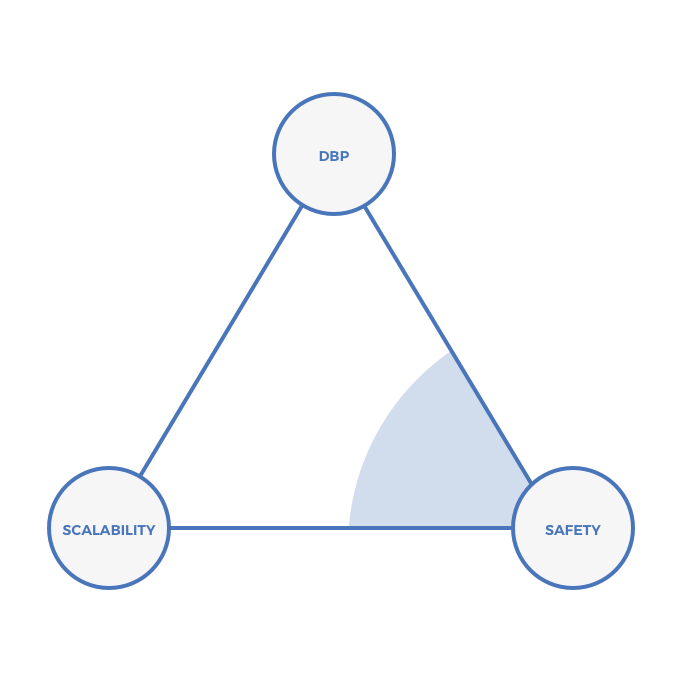
\includegraphics[width=0.5\textwidth]{scalability_triangle_pow}
    \caption{Bitcoin and Ethereum's PoW networks have slow probabilistic time to finality and do not scale well. Mining capacity has high concentration in a small amount of entities, from \cite{scaling-trustless-models}}
    \label{fig:scalability_triangle_pow}
\end{figure}

We proceed to discuss some network level solutions that can improve Ethereum's scalability.

\subsubsection{Proof-of-Stake}
Proof-of-Stake (PoS) is an alternative consensus algorithm where in the place of miners, there are validators who instead of expending computational resources to `mine' a valid block, they stake\footnote{Lock up for an amount of time} their ether and the probability for them to be elected to validate the next block is proportional to their stake. Designing a secure PoS protocol is still under heavy research. The Ethereum Foundation is working on `Casper the Friendly Finality Gadget'\cite{casperffg} which is a hybrid PoW/PoS consensus algorithm that provides block finality\footnote{A block that is finalized cannot be reverted. This is different to traditional PoW which achieves \textit{probabilistic finality}; a block is considered harder to revert the older it is} which combined with the `correct-by-construction Casper the Friendly GHOST'\footnote{Uses the GHOST protocol to choose a chain in the case of a fork.} \cite{caspertfg} will enable a full transition to Proof of Stake. 

\subsubsection{Sidechains}
A sidechain \cite{sidechains} is a blockchain defined by a custom `rule-set' and can be used to offload computations from another chain. Individual sidechains can follow different sets of rules from the mainchain, which means they can optimize for applications that require high speeds or heavy computation, while still relying on the mainchain for issues requiring the highest levels of security. Ethereum's sidechain solution is called `Plasma' \cite{plasma} and involves creating `child-chains' that run their own consensus algorithm with a two-way peg as described in \cite{sidechains}. \textit{Plasma chains} can have more adjustable parameters such as be less decentralized, however the protocol does not allow for the child-chain operator to abuse their power. A more recent Plasma construct is called `Plasma-Cash' \cite{plasmacash} and describes a more efficient way of executing fraud proofs, in the case of a malicious actor in a \textit{Plasma chain}.

\subsubsection{Sharding}
Due to the architecture of the EVM all transactions are executed sequentially on all ethereum nodes. Sharding refers to splitting the process across nodes, so that each full node is responsible only for a shard\footnote{A shard is a part of the blockchain's state} and acts as a light client to the other shards. Sharding is the most complex scaling solution and is still at research stages. It also requires a stable Proof of Stake consensus algorithm to function properly.

\subsubsection{State channels}
Contrary to the previous solutions which still record messages on a blockchain, state channels involves exchange of information `off-chain'. The primary use-case for state channels is micro-transactions between two or more parties. This technique involves exchanging signed messages through a secure communications channel and perform a transaction on the blockchain only when the process is done\footnote{Example: Instead of making 10 transactions worth 0.1 ether each, a transaction is made to open the channel, participants exchange off-chain messages transferring value, and settle or dispute the channel with one more transaction at the end.}.
    
\section{Contract Level Scalability}
In a recent study \cite{DBLP:journals/corr/ChenLLZ17}, after evaluating 4240 smart contracts, it is found that over 70\% of them are under-optimized with respect to gas from the compiler. In this section we explore how gas gets computed in smart contracts and ways we can save on gas and transaction costs.


\subsection{Gas Costs}
An Ethereum transaction's gas costs are split in: % https://ethereum.stackexchange.com/a/29560
\begin{enumerate}
    \item \textbf{Transaction Costs:} The cost of sending data to the blockchain. There are 4 items which make up the full transaction cost:
        \begin{enumerate}
            \item The base cost of a transaction (21000 gas)
            \item The cost of a contract deployment (32000 gas)
            \item The cost for every zero byte of data in a transaction's input (4 gas per zero byte).
            \item The cost of every non-zero byte of data in a transaction's input (68 gas per zero byte)
        \end{enumerate}
    \item \textbf{Execution Costs:} The cost of computational operations which are executed as a result of the the transaction, as described in detail in \cite{ethereum, gas} 
\end{enumerate} 

[INSERT TABLE ON GAS COSTS SHOWING SSTORE ETC]

% bytecontracts includes constructor and general initialisation contracts which is not needed anymore at runtime. The contracts that is sent during deployment (bytecontracts), even excluding the constructor arguments, is - in general - different from the contracts that is stored at that address (the runtimeBytecontracts).


% \input{contracts/opcontracts_table.tex}
Gas costs get translated to transaction fees. As a result, a contract should be designed to minimize its operational gas costs in order to minimize its transaction fees. In addition, as gas is a unit for computational costs, less gas consumed results in less burden on the nodes validating the smart contracts which can lead to better scalability.

From the gas cost table, it can be seen that the most expensive operations involve CREATE\footnote{Used to create a new contract.} and SSTORE operations. The focus of this section will be to explore ways to decrease gas costs on Smart Contracts, either through better practices or by handcrafting optimizations for specific use cases.

It should be noted, that non-standard methods have been proposed for reducing fees incurred by gas costs. A recent construction\cite{gastoken} describes a method of buying gas at low cost periods and saving it in order to spend it when gas prices are higher\footnote{When the network is congested}. The economic implications of gas arbitrage are outside the scope of this Master Thesis. 

General rules that should be followed for saving gas costs:
\begin{enumerate}
    \item Enable compiler optimizations (although can lead to unexpected scenarios \cite{compiler}).
    \item Reuse contracts through libraries\cite{library}.
    \item Setting a variable back to zero refunds 15000 gas through SSTORE, so if a variable is going to be unused it is considered good practice to call `delete' on it. 
    \item Use `bytes32' instead of `string' for strings that are of known size. `bytes32' always fit in an EVM word, while `string' types can be arbitrarily long and thus require more gas for saving their length.
    \item Do not store large amounts of data on a blockchain. It is more efficient to store a hash which can be either proof of the existence of the data at a point in time, or it can be a hash pointing to the full data\footnote{This pattern has been used in combination with IPFS, \url{https://ipfs.io}}
\end{enumerate}

As described in \cite{DBLP:journals/corr/ChenLLZ17} there is a lot of room for further compiler optimizations. Future Solidity compiler versions are addressing some already\footnote{\url{https://github.com/ethereum/solidity/issues/3760}}\footnote{\url{https://github.com/ethereum/solidity/issues/3716}}\footnote{\url{https://github.com/ethereum/solidity/issues/3691}}

The EVM operates on 32 byte words implying that a SSTORE command is needed to store 32 bytes of data. The compiler is able to `tightly pack' data together, which means that 2 128 bit storage variables can be efficiently stored with 1 SSTORE command. The \textit{optimize} flag of the Solidity compiler needs to be activated to access this feature when programming in Solidity.

\begin{figure}[H]
  \begin{subfigure}[b]{\textwidth}
    \centering
    \lstinputlisting[language=Solidity]{contracts/Packing.sol}
  \end{subfigure}

  \begin{subfigure}[b]{\textwidth}
    \centering
    \lstinputlisting{code/solc.txt}
  \end{subfigure}
  \label{fig:struct_optimization}
  \caption{Running the optimizer in storage variables less than 256 bytes results in 2 SSTORE commands instead of 6 which a significant saving in gas costs}
\end{figure}

\subsection{Gas Savings Case Study}
In order to illustrate our findings and compare across different scenarios, we will perform a Solidity benchmarking test based on a use-case of a Solidity Smart Contract which describes a game. The software requirements are: 
\begin{itemize}
    \item A user must be able to register.
    \item A user must be able to create a character with characteristics as function arguments.
    \item A user must be able to get the characteristics of a character.
\end{itemize}% Table describing character characteristics.

\begin{table}[H]
	\centering
	\vspace*{-1ex}
	\scriptsize
	\vspace{-1ex}
	\begin{tabular}{|c|c|c|}
        \hline
        \textbf{Name} & \textbf{Type}  & \textbf{Comment}\\ \hline 
        playerID      & uint16         & Game supports up to 65535 players\\
        creationTime  & uint32         & Game supports timestamps up to 2**32 = 02/07/2106 @ 6:28am (UTC) \\
        class         & uint4          & Game supports up to 16 classes \\
        race          & uint4          & Game supports up to 16 classes \\
        strength      & uint16         & Stats can be up to 65535\\
        agility       & uint16         & Stats can be up to 65535 \\
        wisdom        & uint16         & Stats can be up to 65535 \\
        metadata      & bytes18        & Utilize the rest of the word for metadata \\
        \hline
    \end{tabular}
	\caption{Required variables and size. Sizes add up to 248 bits which can be efficiently stored in a 256 bit word.}
    \label{table:characteristics}
\end{table} % Phrase this better

The size of the variables is selected so that all the information required to describe a `Character' can fit in a 256 bit word.

For each of the following implementations we will examine the deployment gas costs, as well as the gas costs for calling the `CreateCharacter' function:

\begin{enumerate}
    \item Tightly packed structures for setting data
    \item Bit masking encoding for setting data
    \item Bit masking encoding utilizing libraries, influenced by \cite{virtualstruct}.
\end{enumerate}

%% TODO Make contracts appear in some good way. 2 columns, each one for Create/Get character.
The full contracts of each contract can be found in the Appendix. 
For each test described, the optimizer was run 0, 1, 100, 500 and 50000 times.
% \lstinputlisting[language=Solidity]{contracts/GameInterface.sol}
\subsubsection{GameTightlyPacked.sol}
We're utilizing a structure here and by taking advantage of the optimizer packing everything in a word we can perform a full write to structure with only X gas 

% STRUCT DEFINITION | CREATE CHARACTER | GET CHARACTER

% \lstinputlisting[language=Solidity]{contracts/GameTightlyPacked.sol}

\subsubsection{GameByteMasking.sol}

% SHAPE WITH THE MASK HOW CAN IT BE DONE
Here we create a new character by shifting variables. This concept can be though as a `virtualstruct'. Essentially instead of creating a `struct' as Soldiity expects it and let the compiler do the parsing, we do it ourselves. That way, we achieve gas costs which are substantially lower.
% \lstinputlisting[language=Solidity]{contracts/GameByteMasking.sol}
\begin{table}[H]
	\centering
	\vspace*{-1ex}
	\scriptsize
	\caption{Gas costs for Byte masking method wihtout Library}
	\vspace{-1ex}
	\label{gas_bytemasking}
    \begin{tabular}{|c|c|c|c|}
        \hline
        \textbf{Optimizer Runs} & \textbf{Register} & \textbf{CreateCharacter} &  \textbf{Constructor} \\
        0      &    70003 &           66620 &     551800.0 \\
        1      &    69943 &           66365 &     378022.0 \\
        100    &    69811 &           65924 &     402120.0 \\
        500    &    69604 &           65855 &     419559.0 \\
        500000 &    69598 &           65855 &     432537.0 \\
        \hline
    \end{tabular}
\end{table}:

In addition, as we essentially do the optimization ourselves, the deployed bytecode is smaller. 
This is not exactly intuitive, as it'd be expected that the solidity compiler is able to pack everything perfectly. It turns out\footnote{https://github.com/figs999/Ethereum/blob/master/Solc.aComedyInOneAct} that the compiler is not very efficient and as a result this method is far more efficient. With this method we are able to store and fetch all the data in a very efficient way, which costs X\% gas less than the previous implementation. However, this method does not allow for a readable and maintainable interface. In order to export every functionality it is needed to convert the `uint' variables to bytes to perform the bit operations on functions. This creates undesired overhead and thus is avoided.

\subsubsection{GameByteMaskingLib.sol}
It is important to consider code reusability, in the case another developer wanted to develop on the same structure, they should not need to deploy the core functionality of the `Character' structure each time. Utilizing the `using X for Y' syntax, we can export the library's API in a format that is similar to calling functions on struct's in Golang \footnote{\url{ golangtutorials.blogspot.de/2011/06/methods-on-structs.html}}.

The are two ways to export functions when creating Solidity APIs:
\begin{enumerate}
    \item Internal: The library's bytecode is inlined to the main contract's code. This results in larger bytecode during deployment, however each of the contract's function are immediately jumping and returning to the Library's code, like any function. In this case, only the main contract gets deployed.
    \item Public: This is a more complex process:
        \begin{enumerate}
            \item The library contract gets compiled and deployed
            \item The main contract gets compiled and has placeholder slots in the bytecode.
            \item The placeholder gets replaced by the deployed library's address
            \item Any function call that requires the library utilizes the `delegatecall' opcode.
        \end{enumerate}
\end{enumerate}

The usage of the former can be done for separating the code and creating a more well done repository. The latter's usability cna be seen with more general purpose functions such as error-checked functions for mathematic operations. That way, instaed of everyone having to deploy their own version, they can use the already deployed one. The tradeoff comes between deployment costs and calling each function. When the bytecode is inlined, the jumping is done internally, while delegatecall requires additional resources. Finally there is a security gain, such as when everyone uses the same version of an audited library compared to everyone deploying their own. We opt for the internal approach, because cheaper and does not make sense to deploy, i.e. not enough people will care about it.

The final version is split in two files, a library file and a main file. [ EXPLAIN LIBRARIES ]. 
% \lstinputlisting[language=Solidity]{contracts/GameByteMaskingLib.sol}
%\footnote{\url{http://solidity.readthedocs.io/en/v0.4.21/contracts.html#using-for}}

\subsection{Results}
It can be seen that in all cases the optimizer's first iteration creates significant gas savings. However, the more optimizer-runs were done, the more gas cost was spent during deployment, however the cost of `CreateCharacter' went down. Code in Solidity is either optimized for size, and thus costs less to deploy, or for runtime costs, which costs more to deploy but each function costs less \cite{optimizer-tradeoff}.

We described a technique which relies on the compiler's optimizer to pack the data in a struct and do the gas savings, however is simpler and more elegant. The second and third technique are more complex and allow for further gas optimizations. The second technique is more efficient however lacks reusability and is less maintanable. On the other hand, utilizing libraries however we can export a user-friendly API for reusing our code for anyone who has the same use case as us. This technique will be utilized in the Design and implementation section.